\documentclass{article}
\usepackage[utf8]{inputenc}
\usepackage{enumitem}
\usepackage{graphicx}
\usepackage{float}


\begin{document}

\newpage
\title{Digital Watermarking}

	
\newpage
\tableofcontents

\newpage

\section{Subject}

The project's aim is to implement and compare 2 methods of the digital watermarking. Technologies chosen by us are: LSB and Patchwork.
Analysis will be focused on main areas of watermarking which are: transformation, distortion, compression.. //todo: dopisac jakie jeszcze. 

\section{State of art}

Digital watermarking in general is a kind of marker embedded in a noise-tolerant signal. The most popular kinds of the signals which allow watermarking are images, videos, audio. Typically used for identifying ownership and mark copyrights. A digital watermark does not change the size of the carrier signal.
Example of watermark.
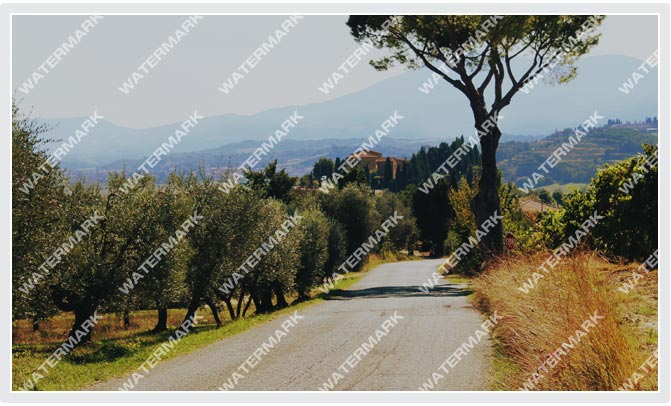
\includegraphics{ex.png}
.
.
.

\begin{enumerate}
	\item Spatial domain techniques - directly add the watermark to pixel values - exploit Human Visual System for hiding the data
	\item Transformed domain techniques - add the watermark to the coefficients of a full-frame transform (DFT, DCT, Mellin, Radon, Fresnell)
	\item Hybrid techniques
\end{enumerate}

\section{Project scope}

In the following subchapters, 

	\subsection{Goal}
	The main goal of the project is to prepare simple application with both of the algorithms implemented. Our tasks were focused on proper algorithm implementation rather than on user interface. We were trying...
	
	\subsection{Communication}
	Communication of team members took place remotely using Trello (an internet
	application for project management) and Facebook Messenger (messenger on a social
	networking site). After the division of tasks through Trello, each member could take on	a specific task and present the progress of the work and the final effects of the project stages on an ongoing basis. Important point of communication were team meetings, where we could discuss problems related to the project implementation and solve difficult tasks more efficient. The source code of the application has been managed remotely using the GitHub repository.
	
	\subsection{Features}

	
	\subsection{Requirements}
\section{Techniques and Technologies}
	
	\begin{itemize}
		\item Python 3.7
		\item NumPy
		\item scikit-image
		\item algorithms: \begin{enumerate}
			\item LSB – Least Significant Bit
			\item Patchwork techniqe
		\end{enumerate}
	\end{itemize}
	
\section{Milestone and project plan}

	\subsection{Team members}
	
	\begin{itemize}
		\item Bartosz Gardziejewski
		\item Rafał Gradkowski
		\item Łukasz Obrebski
		\item Paweł Zaborowski
	\end{itemize}

	\subsection{Project plan}
	
	Out team have splitted into topic groups:
	
	\begin{enumerate}
		\item LSB implementation
		\item Patchwork implementation
		\item Documentation work
	\end{enumerate}
	

	\subsection{Gantt Chart}
	
	\begin{itemize}
	

	\item 11.10.19 – Setup of Trello \& GitHub
	\item 17.10.19 – Project Kick OFF (first presentation)
	\item 14.11.19 – Literature analysis, working Python environment, beginnings of a documentation
	\item 28.11.19 – Implementation of embedding digital watermark in images using both algorithms
	\item 12.12.19 – Implementation of decoding digital watermark in images using both algorithms
	\item 09.01.20 – Juxtaposition and comparison of results
	\item 16.01.20 – Project closure (Final presentation, project demo, documentation)
	\end{itemize}
	
	\subsection{}
\section{Results}

		
	Example:
	
\includegraphics{python.png}
	
\includegraphics{watermarked_python.png}
	
	When we look at background of the black area with "python" word we are able to se generated watermark.


	\subsection{1}
	
	LSB pros and cons:
	\begin{itemize}
		
		\item Resistance to geometric transformations, like cropping, stretching or rotating 
		\item High capacity of watermark
		\item Can be easily destroyed by distortions or gamma changes

	
	
	\end{itemize}	
	
	\subsection{2}
	
	Patchwork pros and cons
	
	\begin{itemize}
		\item Resistance to cropping and to gamma and tone scale corrections
		\item The detector doesn’t require the original cover image to determine whether the image has been watermarked.
		\item Can be destroyed by any affine transformation, like translation, rotation or scaling
	\end{itemize}
	
\section{Conclusions}

	

\end{document}